\chapter{Обзор основных подходов для реализации микросервисов}
\section{Обзор микросервисной архитектуры}

Представление о микросервисах родилось в 2005 году из подхода SOA путем обобщения философии UNIX для веб-компонент.
Веб-сервисы сопоставляются независимым программам, комбинация которых осуществляется с помощью сетевого транспорта данных по аналогии с именованными и неименованными UNIX каналами.
В отличие от SOA микросервисы не фокусируются на конкретных форматах передачи данных, как SOAP, 
а дают представление о том, как должны коммуницировать сервисы, чтобы при сохранении слабой связности компонент поддерживать устоявшийся контракт обмена информацией \cite{micro-1}.

В современной литературе не существует одного конкретного определения микросервиса. 
Обычно микросервисы определяют через различные критерии соответствия распределенной системе с низкой связностью ее отдельных компонент.

Большое внимание в теории микросервисов уделяется вопросам масштабируемости. 
Для всестороннего описания масштабируемости в контексте разработки распределенных систем вводится понятие куба масшабируемости \cite{scalability} (Рисунок \ref{fig:cube}).

\begin{figure}[H]
    \centering
    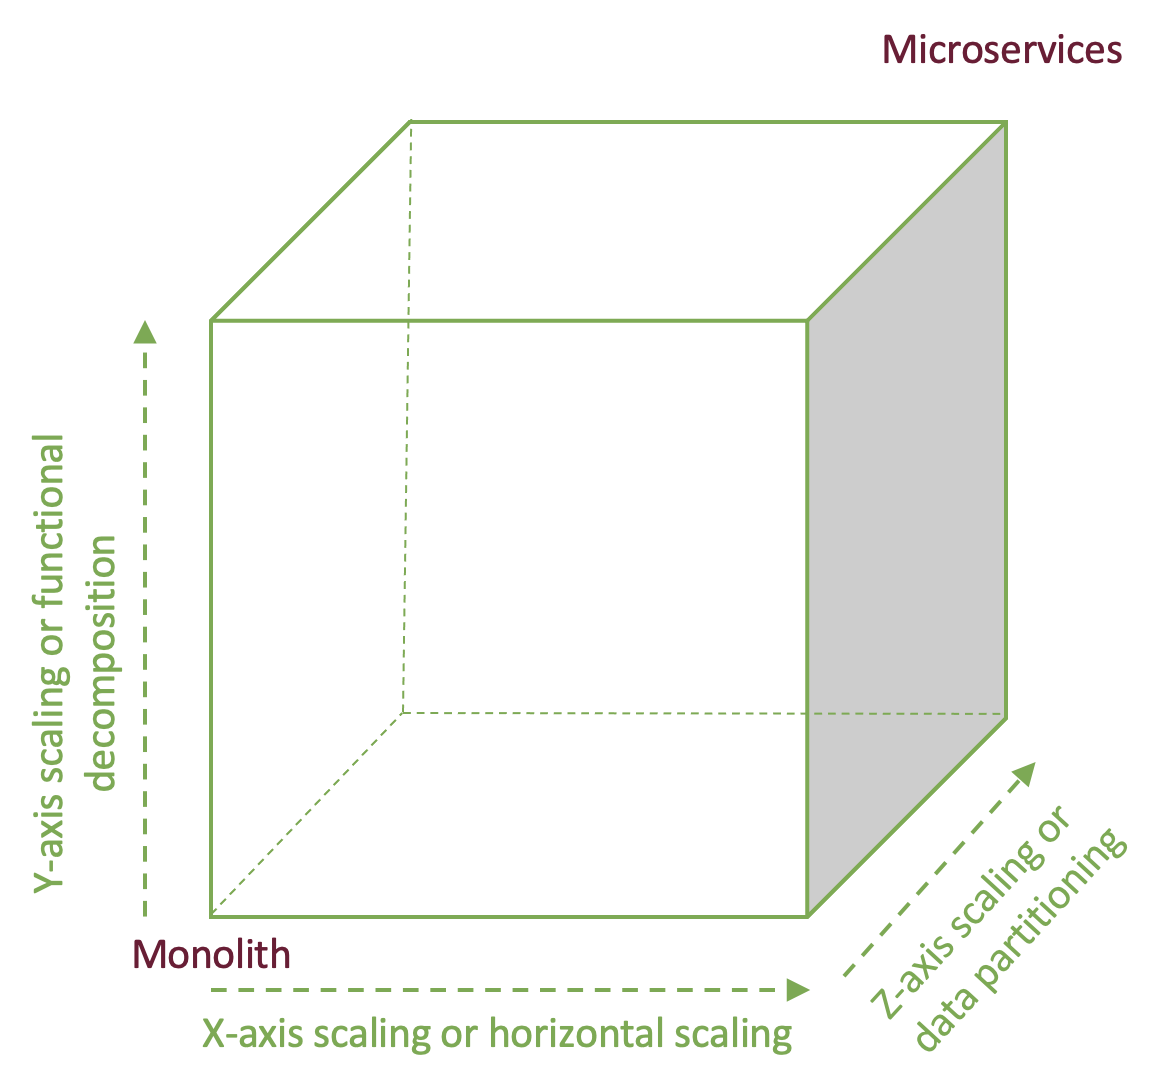
\includegraphics[width=0.5\linewidth]{img/cube.png}
    \caption{Куб масштабируемости}
    \label{fig:cube}
\end{figure}

Эта модель определяет три направления для масштабирования приложений: $X$, $Y$ и $Z$.

Масштабирование по оси X часто применяют в монолитных приложениях. 
Запускается несколько экземпляров программы, размещенных за балансировщиком нагрузки. 
Балансировщик распределяетзапросы между $N$ одинаковыми экземплярами. 
Это распространенный способ улучшить
производительность и стабильность приложения.

Масштабирование по оси $Z$ тоже предусматривает запуск нескольких экземпляров
монолитного приложения, но в этом случае, в отличие от масштабирования по
оси $X$, каждый экземпляр отвечает за определенное подмножество данных.
Маршрутизатор, выставленный впереди, задействует атрибут запроса, чтобы на
править его к подходящему экземпляру. 

Масштабирование по осям $X$ и $Z$ увеличивает производительность и стабильность приложения.
Но ни один из этих подходов не решает проблем с усложнением кода и процесса раз
работки. Чтобы справиться с ними, следует применить масштабирование по оси $У$,
или функциональную декомпозицию. То, как это работает, показано на рисунке \ref{fig:y}.
\begin{figure}[H]
    \centering
    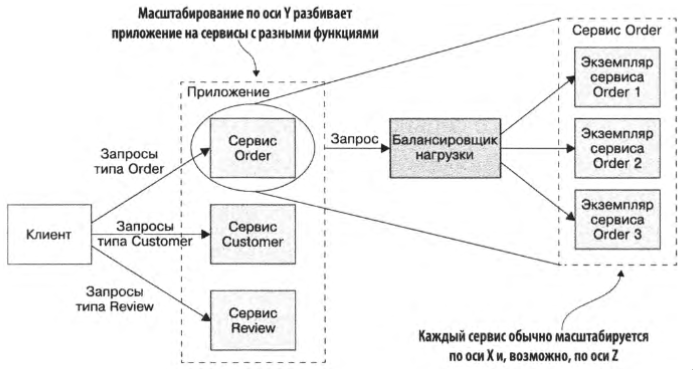
\includegraphics[width=0.8\linewidth]{img/y.png}
    \caption{Пример декомпозиции приложения через отдельные сервисы}
    \label{fig:y}
\end{figure}

Таким образом, сервис — это приложение, реализующее узкоспециализированные функции, такие как управление заказами, управление клиентами и т. д. 
Сервисы масштабируются по оси $X$, некоторые из них могут использовать также ось $Z$. Например,
сервис Order (Рисунок \ref{fig:y}) имеет несколько копий, нагрузка на которые балансируется.
Одно из обобщенных определение микросервисной архитектуры (или микросервисов)
звучит так: это стиль проектирования, который разбивает приложение на отдельные
сервисы с разными функциями. Заметим, что размер здесь вообще не упоминается.
Главное, чтобы каждый сервис имел четкий перечень связанных между собой обязанностей.

Микросервисная архитектура имеет следующие преимущества:
\begin{itemize}
    \item Она делает возможными непрерывные доставку и развертывание крупных, сложных приложений.
    \item Сервисы получаются небольшими и простыми в обслуживании.
    \item Сервисы развертываются независимо друг от друга.
    \item Сервисы масштабируются независимо друг от друга.
    \item Микросервисная архитектура обеспечивает автономность команд разработчиков.
    \item Она позволяет экспериментировать и внедрять новые технологии.
    \item В ней лучше изолированы неполадки других сервисов.
\end{itemize}

Одна из проблем, возникающих при использовании микросервисной архитектуры, связана с отсутствием конкретного, хорошо описанного алгоритма разбиения
системы на микросервисы. 
Что означает, что эта часть данной методологии, не имеет формального описания \cite{micro-1}. 

В связи с этим также выделяют понятие распределенного монолита.

Распределенным монолитом называют набор связанных между собой сервисов, которые необходимо развертывать вместе. Распределенному монолиту присущи недостатки
как монолитной, так и микросервисной архитектуры.

Еще один недостаток микросервисной архитектуры состоит в том, что при создании
распределенных систем возникают дополнительные сложности для разработчиков. 
Сервисы должны использовать механизм межпроцессного взаимодействия.

Это сложнее, чем вызывать обычные методы в общей памяти приложения. 
К тому же код должен уметь
справляться с частичными сбоями и быть готовым к недоступности или высокой
латентности удаленного сервиса.
Реализация сценариев, охватывающих несколько сервисов, требует применения
дополнительных технологий. 

Для реализации надлежащего уровня изоляции между микросервисами применяется паттерн database per service.
В этом случае каждый микросервис имеет собственную базу данных при необходимости холодного хранилища данных. 
Это позволяет вносить правки в функциональность сервиса без риска сломать функциональность другого сервиса и привлечения других команд для согласования изменений, 
а также позволяет просто оценивать время ответов и нагрузку для каждого из сервисов по отдельности, что сложно осуществимо при использовании общих ресурсов.

Несмотря на вышеперечисленные преимущества упомянутого паттерна, database per service затрудняет реализацию комбинированных транзакций и запросов. 
Подобные операции по модификации данных в разных инстансах баз данных называют распределенными транзакциями.
Возникновение распределенных транзакций в архитектуре приложения налагает ограничения на повторные запросы и хеджирование, что налагает
ограничения на применение практик по повышению надежности системы, поскольку при повторных неиндемпотентных запросах или прерванных запросах на запись в несколько баз данных
может быть нарушена консистентность данных.
Для решения подобных проблем внедряются отдельные протоколы координации запросов в базы данных.

Примером подобного протокола является 2PC (two phase commit) -- двухфазный коммит. Этот протокол предполагает
наличие надежного координатора, который предоставляет общую точку синхронизации для разных сервисов, и откатывает изменения
во всех базах при возникновении ошибок в одном из узлов.
\begin{figure}[H]
    \centering
    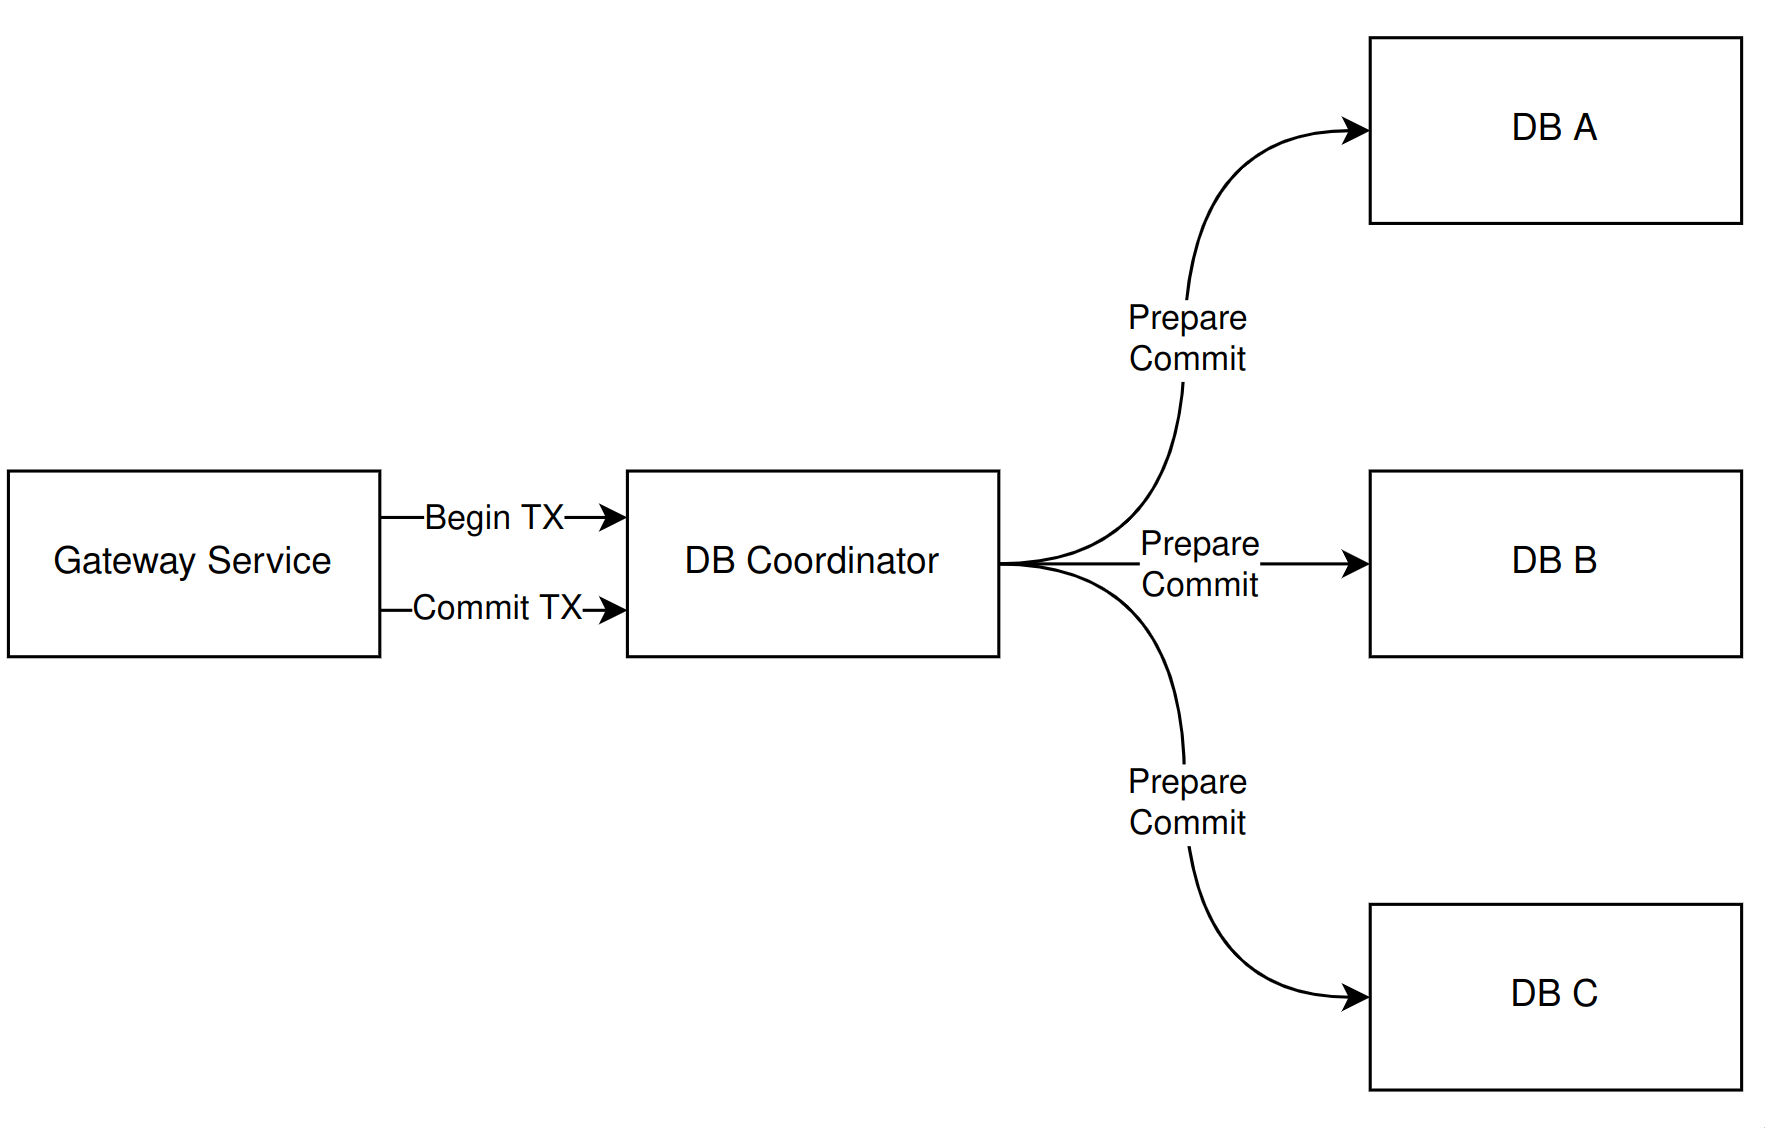
\includegraphics[width=0.8\linewidth]{img/2pc.png}
    \caption{Пример декомпозиции приложения через отдельные сервисы}
    \label{fig:y}
\end{figure}

Несмотря на то, что протокол был разработан в 70-ые годы, он до сих используется в современных приложениях, например,
менеджером транзакций Narayana для платформы Spring. Многие базы данных также предоставляют достаточные механизмы транзакций, которые
требуются для реализации данного протокола. В данном случае достигается максимально возможная консистентность данных, однако
необходимость в отдельном узле синхронизации снижает производительность, усложняет масштабирование, а также плохо получается применить
протокол для нереляционных баз данных.

Также IDE и другие инструменты разработки рассчитаны на создание монолитных
приложений и не обеспечивают явной поддержки распределенных приложений.
Написание автоматических тестов, затрагивающих несколько сервисов, — непростая
задача. 

Все эти проблемы характерны для микросервисной архитектуры. 
Вдобавок микросервисная архитектура существенно усложняет администрирование. В промышленной среде приходится иметь дело с множеством экземпляров
разнородных сервисов, для успешного развертывания которых требуется
высокая степень автоматизации.

Еще одна проблема микросервисной архитектуры связана с тем, что развертывание
функций, охватывающих несколько сервисов, требует тщательной координации
действий разных команд разработки и создание плана выкатки. Для сравнения: в монолитной архитектуре возможно параллельное обновление для нескольких компонентов.

Еще одна трудность связана с решением о том, на каком этапе жизненного цикла
приложения следует переходить на микросервисную архитектуру. Часто во время
разработки первой версии система не сталкивается с проблемами, которые эта
архитектура решает \cite{kaban}. 

Более того, применение сложного, распределенного метода
проектирования замедлит разработку. Для стартапов, которым обычно важнее всего
как можно быстрее развивать свою бизнес-модель и сопутствующее приложение, это
может вылиться в непростую дилемму. Использование микросервисной архитектуры делает выпуск начальных версий довольно трудным. Стартапам почти всегда
лучше начинать с монолитного приложения.

Однако со временем возникает другая проблема: как справиться с возрастающей сложностью. Это подходящий момент для того, чтобы разбить приложение
на микросервисы с разными функциями. Рефакторинг может оказаться непростым
из-за запутанных зависимостей. В связи с этим к переходу на них следует отнестись очень серьезно. Но обычно для сложных проектов, таких как пользовательские веб- или
SaaS-приложения, это правильный выбор. Такие общеизвестные сайты, как eBay, Amazon.com, Groupon и Gilt, в свое время перешли на микросервисы с монолитной архитектуры.

При использовании микросервисов приходится иметь дело с множеством проблем, связанных с проектированием и архитектурой.
К тому же многие из этих
проблем имеют несколько решений со своими плюсами и минусами. Единого
идеального решения не существует \cite{micro-1}.